\documentclass{article}
\usepackage{tikz}
\usetikzlibrary{matrix}

\begin{document}

\begin{center}
    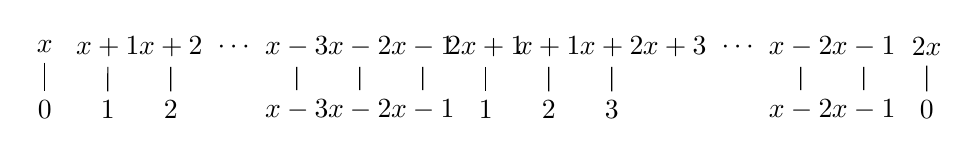
\begin{tikzpicture}[scale=0.8]
        % Define nodes
        \node (a) at (0,0) {$x$};
        \node (b) at (1,0) {$x+1$};
        \node (c) at (2,0) {$x+2$};
        \node (d) at (3,0) {$\cdots$};
        \node (e) at (4,0) {$x-3$};
        \node (f) at (5,0) {$x-2$};
        \node (g) at (6,0) {$x-1$};
        
        \node (h) at (0,-1) {$0$};
        \node (i) at (1,-1) {$1$};
        \node (j) at (2,-1) {$2$};
        
        \node (k) at (4,-1) {$x-3$};
        \node (l) at (5,-1) {$x-2$};
        \node (m) at (6,-1) {$x-1$};
        
        % Draw edges
        \draw (a) -- (h);
        \draw (b) -- (i);
        \draw (c) -- (j);
        \draw (e) -- (k);
        \draw (f) -- (l);
        \draw (g) -- (m);
        
        % Repeat pattern for the second part of the image
        \begin{scope}[xshift=7cm]
            \node (a') at (0,0) {$2x+1$};
            \node (b') at (1,0) {$x+1$};
            \node (c') at (2,0) {$x+2$};
            \node (d') at (3,0) {$x+3$};
            \node (e') at (4,0) {$\cdots$};
            \node (f') at (5,0) {$x-2$};
            \node (g') at (6,0) {$x-1$};
            \node (h') at (7,0) {$2x$};
            
            \node (i') at (0,-1) {$1$};
            \node (j') at (1,-1) {$2$};
            \node (k') at (2,-1) {$3$};
            
            \node (l') at (5,-1) {$x-2$};
            \node (m') at (6,-1) {$x-1$};
            \node (n') at (7,-1) {$0$};
            
            \draw (a') -- (i');
            \draw (b') -- (j');
            \draw (c') -- (k');
            \draw (f') -- (l');
            \draw (g') -- (m');
            \draw (h') -- (n');
        \end{scope}
    \end{tikzpicture}
\end{center}

The perfect linear realizations $\mathbf{g_1}$ and $\mathbf{g_2}$ for $\{ (x-1)^{x-1}, x^x \}$ and $\{ x^{x+2}, (x+1)^{x-1} \}$ respectively.

\end{document}